\documentclass[letterpaper, 10 pt, conference]{article} 
\usepackage[english]{babel}
\usepackage{amsmath,amssymb,amscd,amsthm} % variety of useful math macros
\usepackage[inner=1.5 cm, outer = 1.5 cm, top=1 cm, bottom = 1.5 cm]{geometry}
\usepackage{subcaption}
%Para insertar imágenes
\usepackage{graphicx}
\usepackage[dvipsnames]{xcolor}
\usepackage{listings}
\usepackage[utf8]{inputenc}
\usepackage{hyperref}
%Para crear diagramas
%\usepackage{tikz} 

\newcommand\N{\ensuremath{\mathcal{N}}}

\title{Exploring the text distribution of Nietzsche's \it{Antichrist}}
\author{G. Palafox}

\lstset{ 
	basicstyle=\footnotesize,        % the size of the fonts that are used for the code
	breakatwhitespace=false,         % sets if automatic breaks should only happen at whitespace
	breaklines=true,                 % sets automatic line breaking
	showspaces=false,                % show spaces everywhere adding particular underscores; it overrides 
	showstringspaces = false,
	stringstyle=\color{MidnightBlue},     % string literal style
	backgroundcolor=\color{White},   
}

\begin{document}

\maketitle

\begin{abstract}
An elementary text analysis of Nietzsche's \textit{The Antichrist} \cite{antichrist} is performed. The distribution of some of the obtained data is estimated. 
\end{abstract}

\section{Introduction}
A text analysis of Nietzsche's \textit{The Antichrist} \cite{antichrist} is performed. We find the frequency of common words, and explore the lengths of sentences in the text. We try to find the distribution of this data, or simulate it if we cannot find a fitting common distribution. Additionally, we compare a network representation of the book with a random network having the same degree distribution.

\section{Text analysis and distributions}
The text extraction and analysis is performed in a Jupyter \cite{jupyter} notebook running R \cite{R} version 4.0.0\footnote{The script and a Jupyter \cite{jupyter} notebook detailing our analysis and graphics creation, can be found at \url{https://github.com/palafox794/AppliedProbabilityModels/tree/master/Assignment3}}. The book is downloaded directly from Project Gutenberg's site using R's \texttt{gutenbergr} library. The book downloaded starts with an introduction by the translator, which we omitted from the analysis, as the intention was to study the author's words.

First we obtain two elements of the text: the length of its sentences, and the frequency of the words appearing in it. We discard so called stop-words, and keep only the most frequent words (those appearing over eight times).  We create a histogram of the sentences' length, that can be seen in Figure \ref{fig:sentences_histogram}. From our knowledge of discrete distributions, we infer these data has a geometric distribution. We use R's function \texttt{fitdistr} from the \texttt{MASS} library to try and fit the data to a geometric distribution, obtaining a parameter $p = 0.36$. We generate a thousand pseudo-random numbers with geometric distribution and $p = 0.36$, and plot a histogram of these values, as seen in Figure \ref{fig:rgeom_hist}. Observing these two histograms side-by-side in Figure \ref{fig:histograms}, we conclude the length of the sentences has a geometric distribution with $p=0.36$.

In the case of the word frequency, which is plotted in Figure \ref{fig:barplot_book}, the function \texttt{fitdistr} does not give as good of a match. In this case, we pseudo-randomly select words from the text, aiming to obtain a distribution similar to the actual one. To do this, we do the following. We interpret the bar plot as a probability mass function (prior to normalizing the area to be one). Then, we partition the words in groups according to the frequency of which they occur. We calculate the area of each of these groups, relative to the total area, to partition get a partition $p_0 = 0, p_1, \dots, p_8, p_9 = 1$ of the unit interval . Finally, we generate a pseudo-randomly generated number $p$, and select a word pseudo-randomly from group $k$ if $p_{k-1} \leq p \leq p_k$. A bar plot showing the frequency of the randomly generated words is shown in Figure \ref{fig:barplot_random}. It can be compared to the actual frequency of words in the text in Figure \ref{fig:barplots}. Additionally, Table \ref{tab:wordfreq} shows the most frequent words from both the text and our random selection, and Figure \ref{fig:boxplot} shows a boxplot comparing these two data sets.

\begin{table}[t]
	\caption{Word frequency }
	\begin{subtable}{0.45\textwidth}
		\centering
		\caption{Frequency of words in the book}
	\begin{tabular}{lr}
		\hline
		words & freq \\ 
		\hline
		god & 172 \\ 
		life &  96 \\ 
		christian &  90 \\ 
		christianity &  89 \\ 
		world &  78 \\ 
		truth &  54 \\ 
		\hline
	\end{tabular}
	\label{tab:barplot_words}
	\end{subtable}
	\hfill
	\begin{subtable}{0.45\textwidth}
		\centering
		\caption{Frequency of pseudo-randomly selected words from book}
		\begin{tabular}{lr}
			\hline
			rand\_words & Freq \\ 
			\hline
			god & 162 \\ 
			world & 124 \\ 
			life &  89 \\ 
			christian &  83 \\ 
			christianity &  82 \\ 
			sort &  60 \\ 
			\hline
		\end{tabular}
		\label{tab:barplot_rand_words}
	\end{subtable}
	\label{tab:wordfreq}
\end{table}


 \begin{figure}
 	\centering
 	\begin{subfigure}[b]{0.45\linewidth}
 		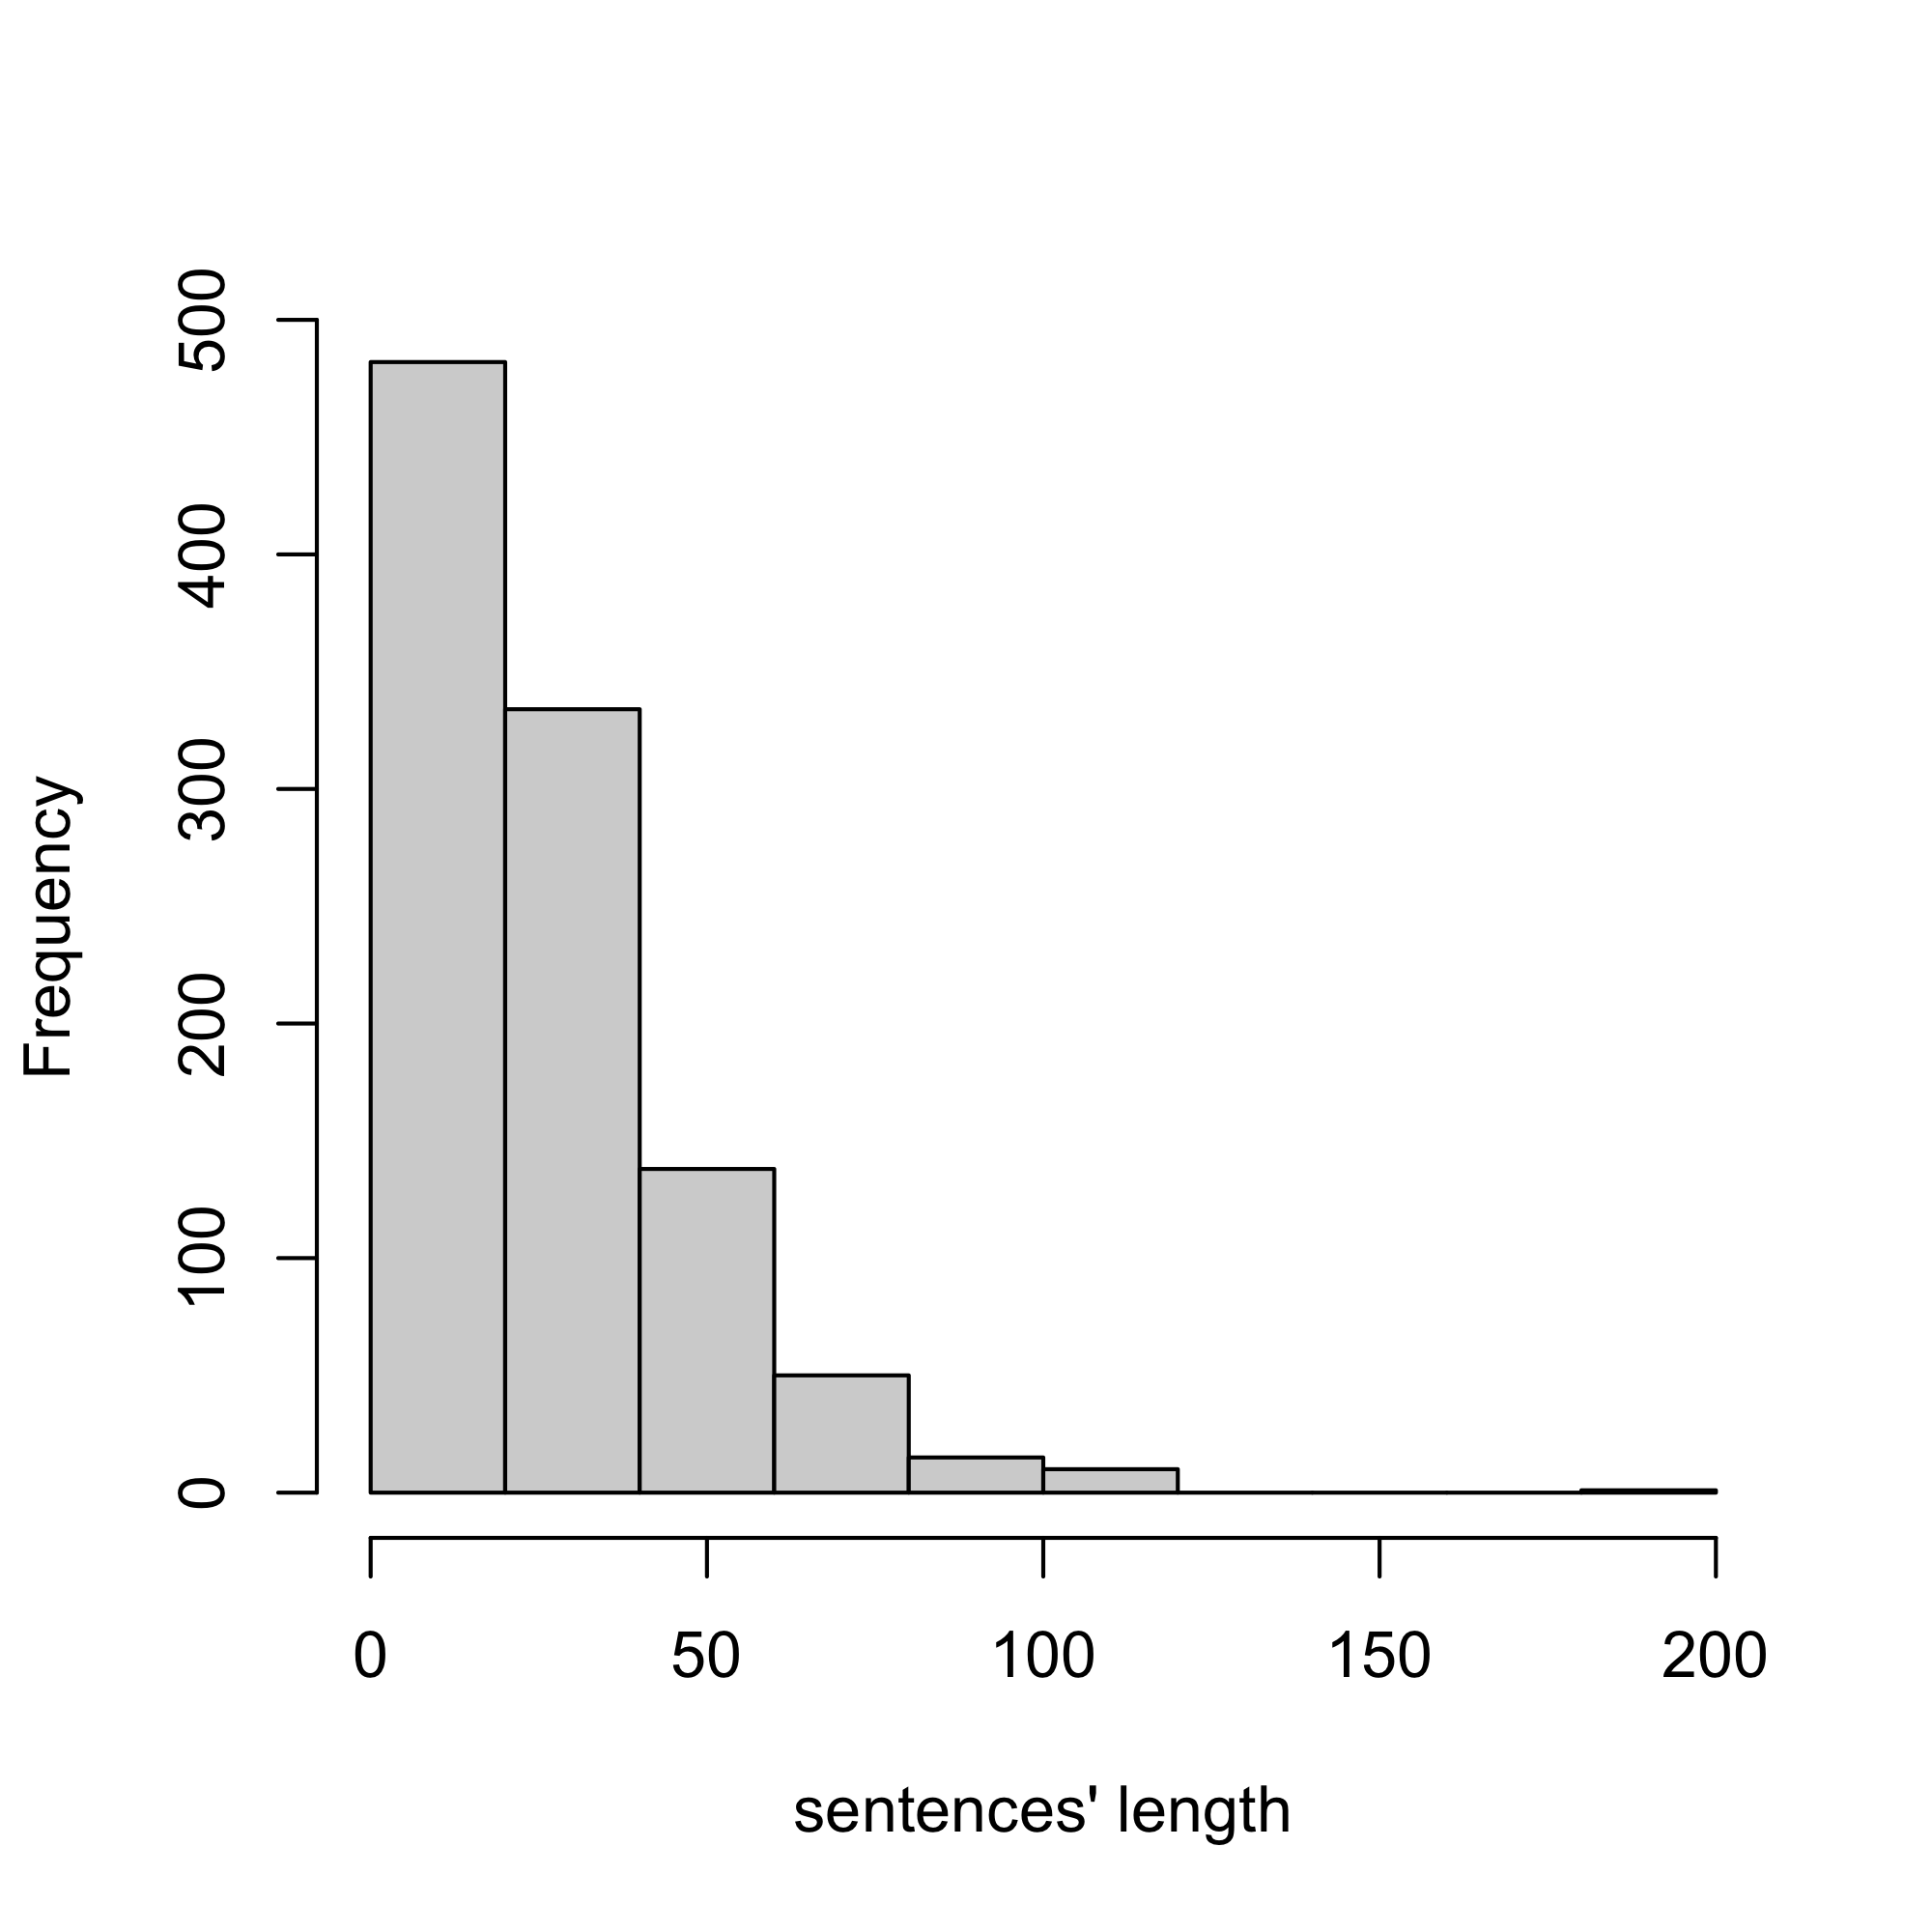
\includegraphics[width=\linewidth]{sentence_length_histogram.png}
 		\caption{Histogram of sentences' length.}
 		\label{fig:sentences_histogram}
 	\end{subfigure}
 	\begin{subfigure}[b]{0.45\linewidth}
 	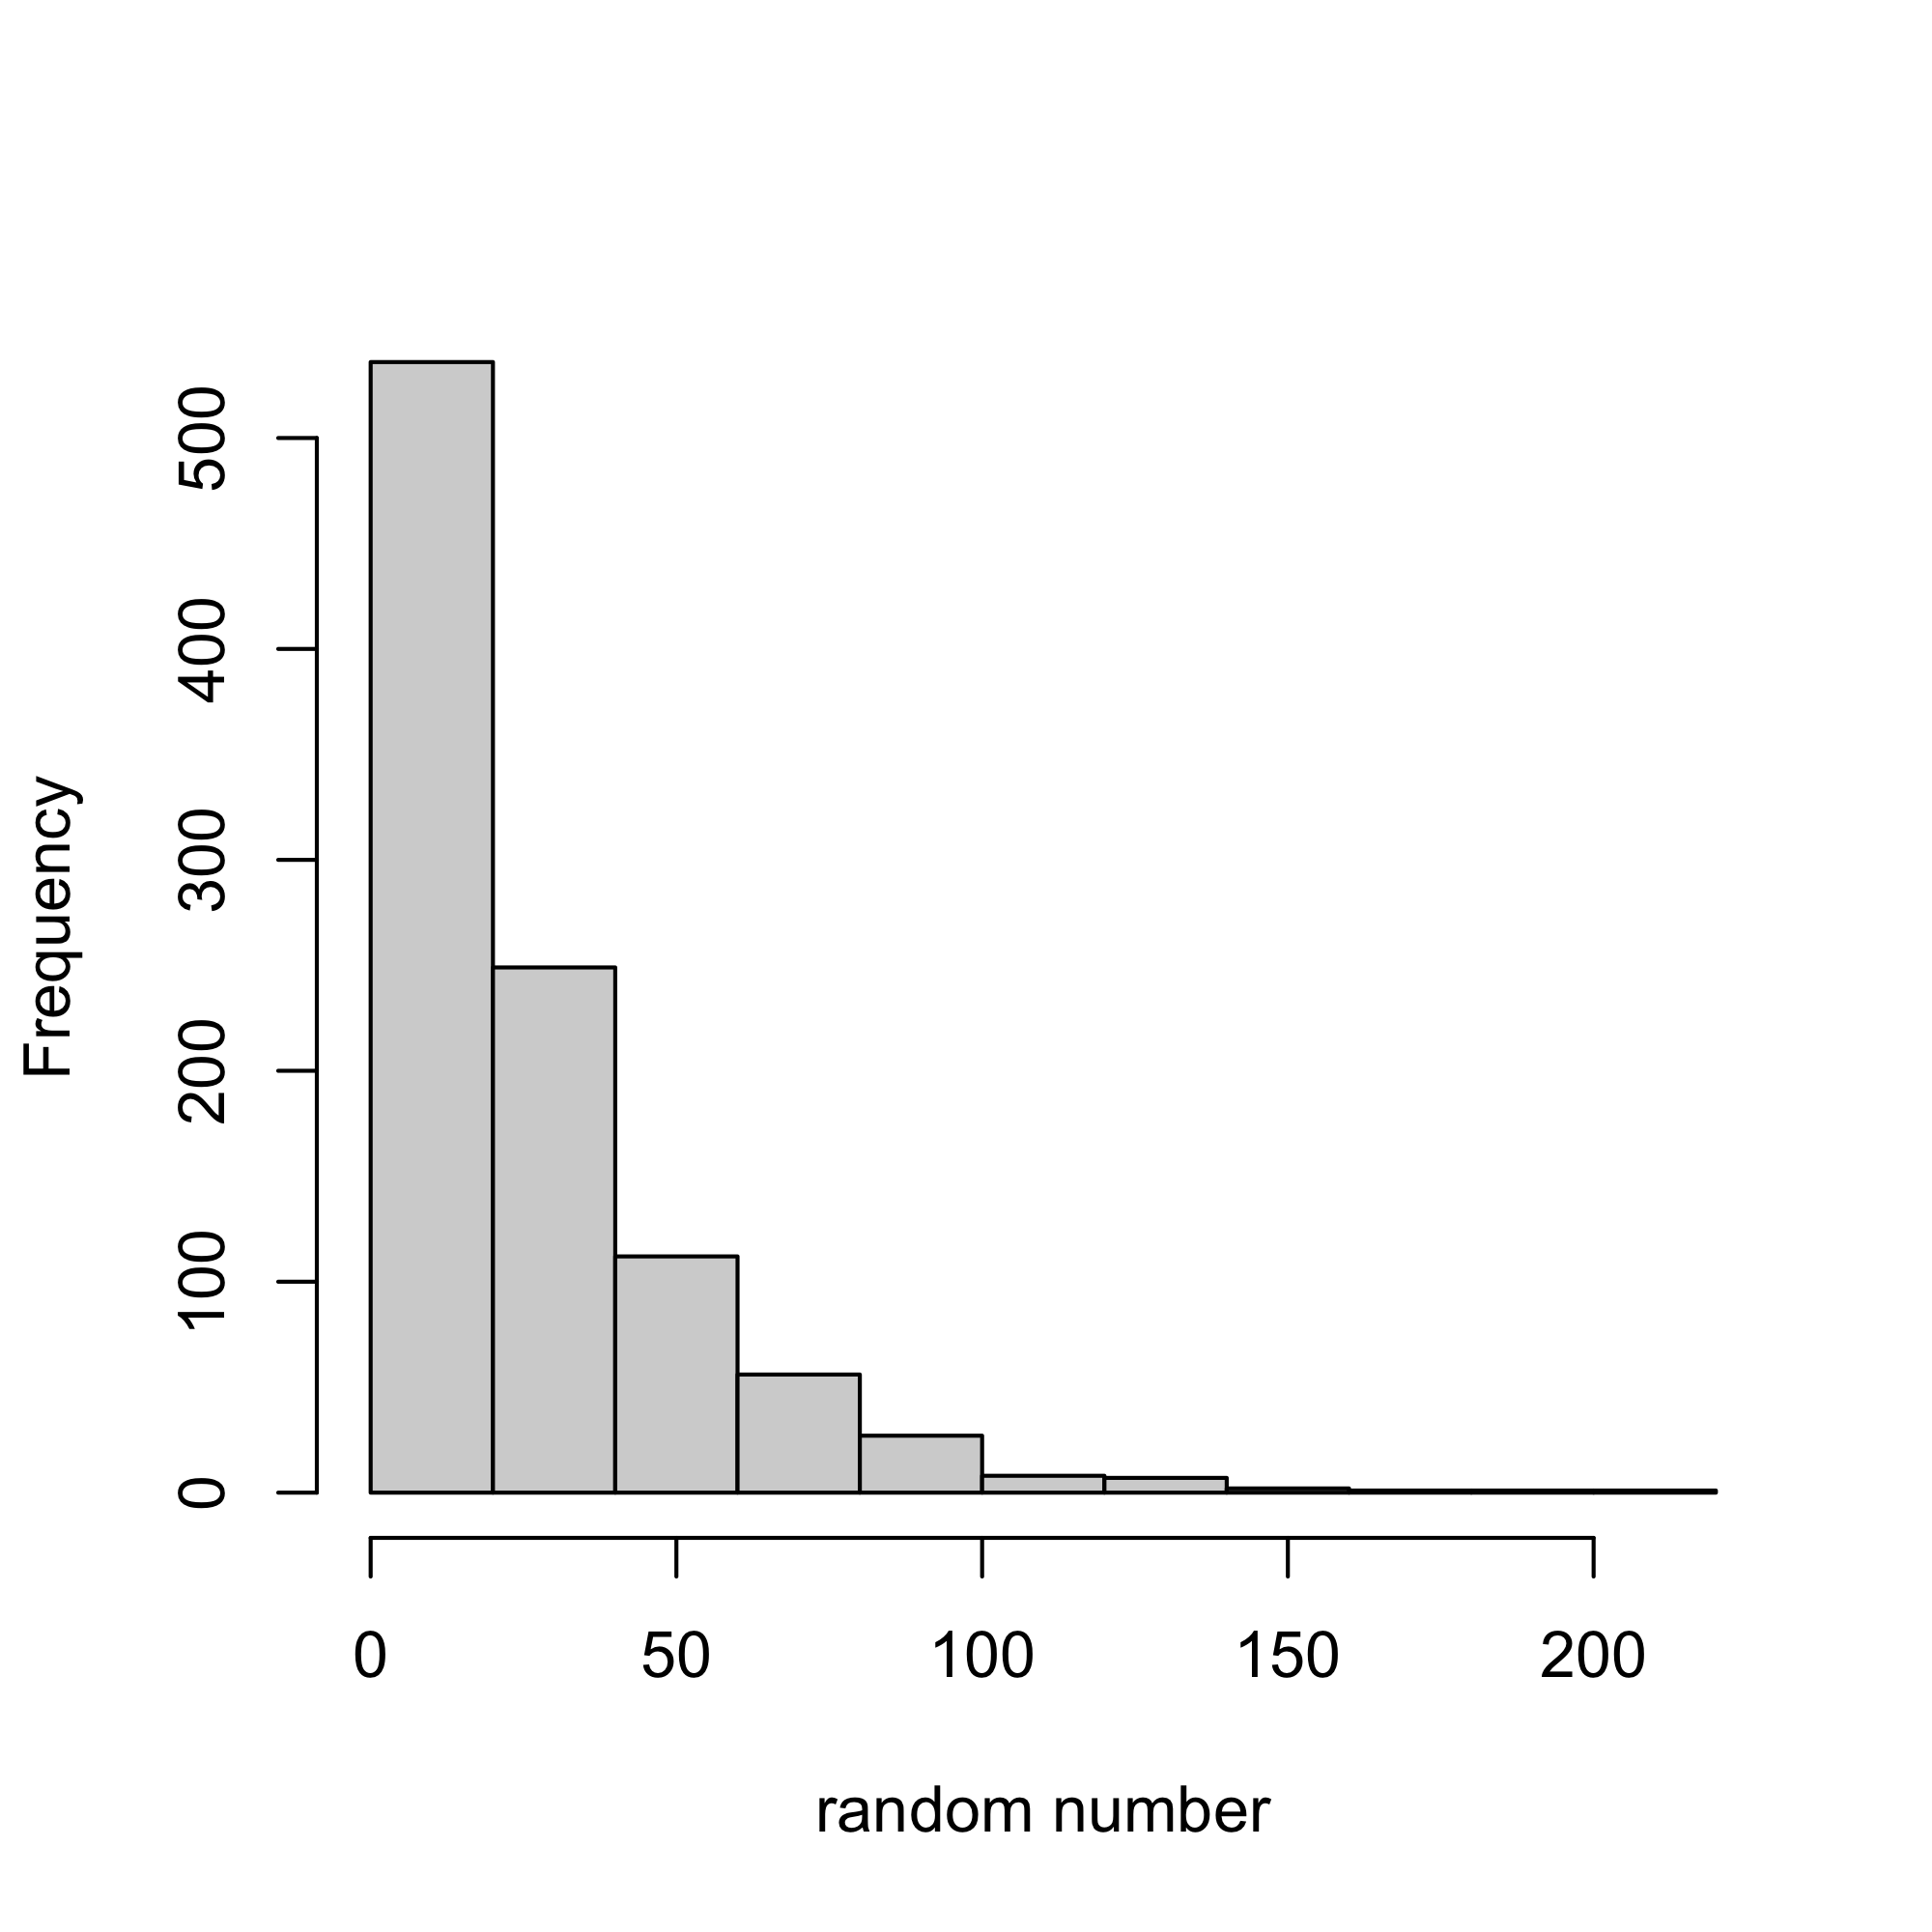
\includegraphics[width=\linewidth]{rgeom_histogram.png}
  	\caption{Histogram of 1000 words with distribution $\mathrm{Geo}(0.36)$.}
  	\label{fig:rgeom_hist}
	 \end{subfigure}
  	\caption{Sentences' length distribution.} 
 	\label{fig:histograms}
 \end{figure}


 \begin{figure}
	\centering
	\begin{subfigure}[b]{0.45\linewidth}
		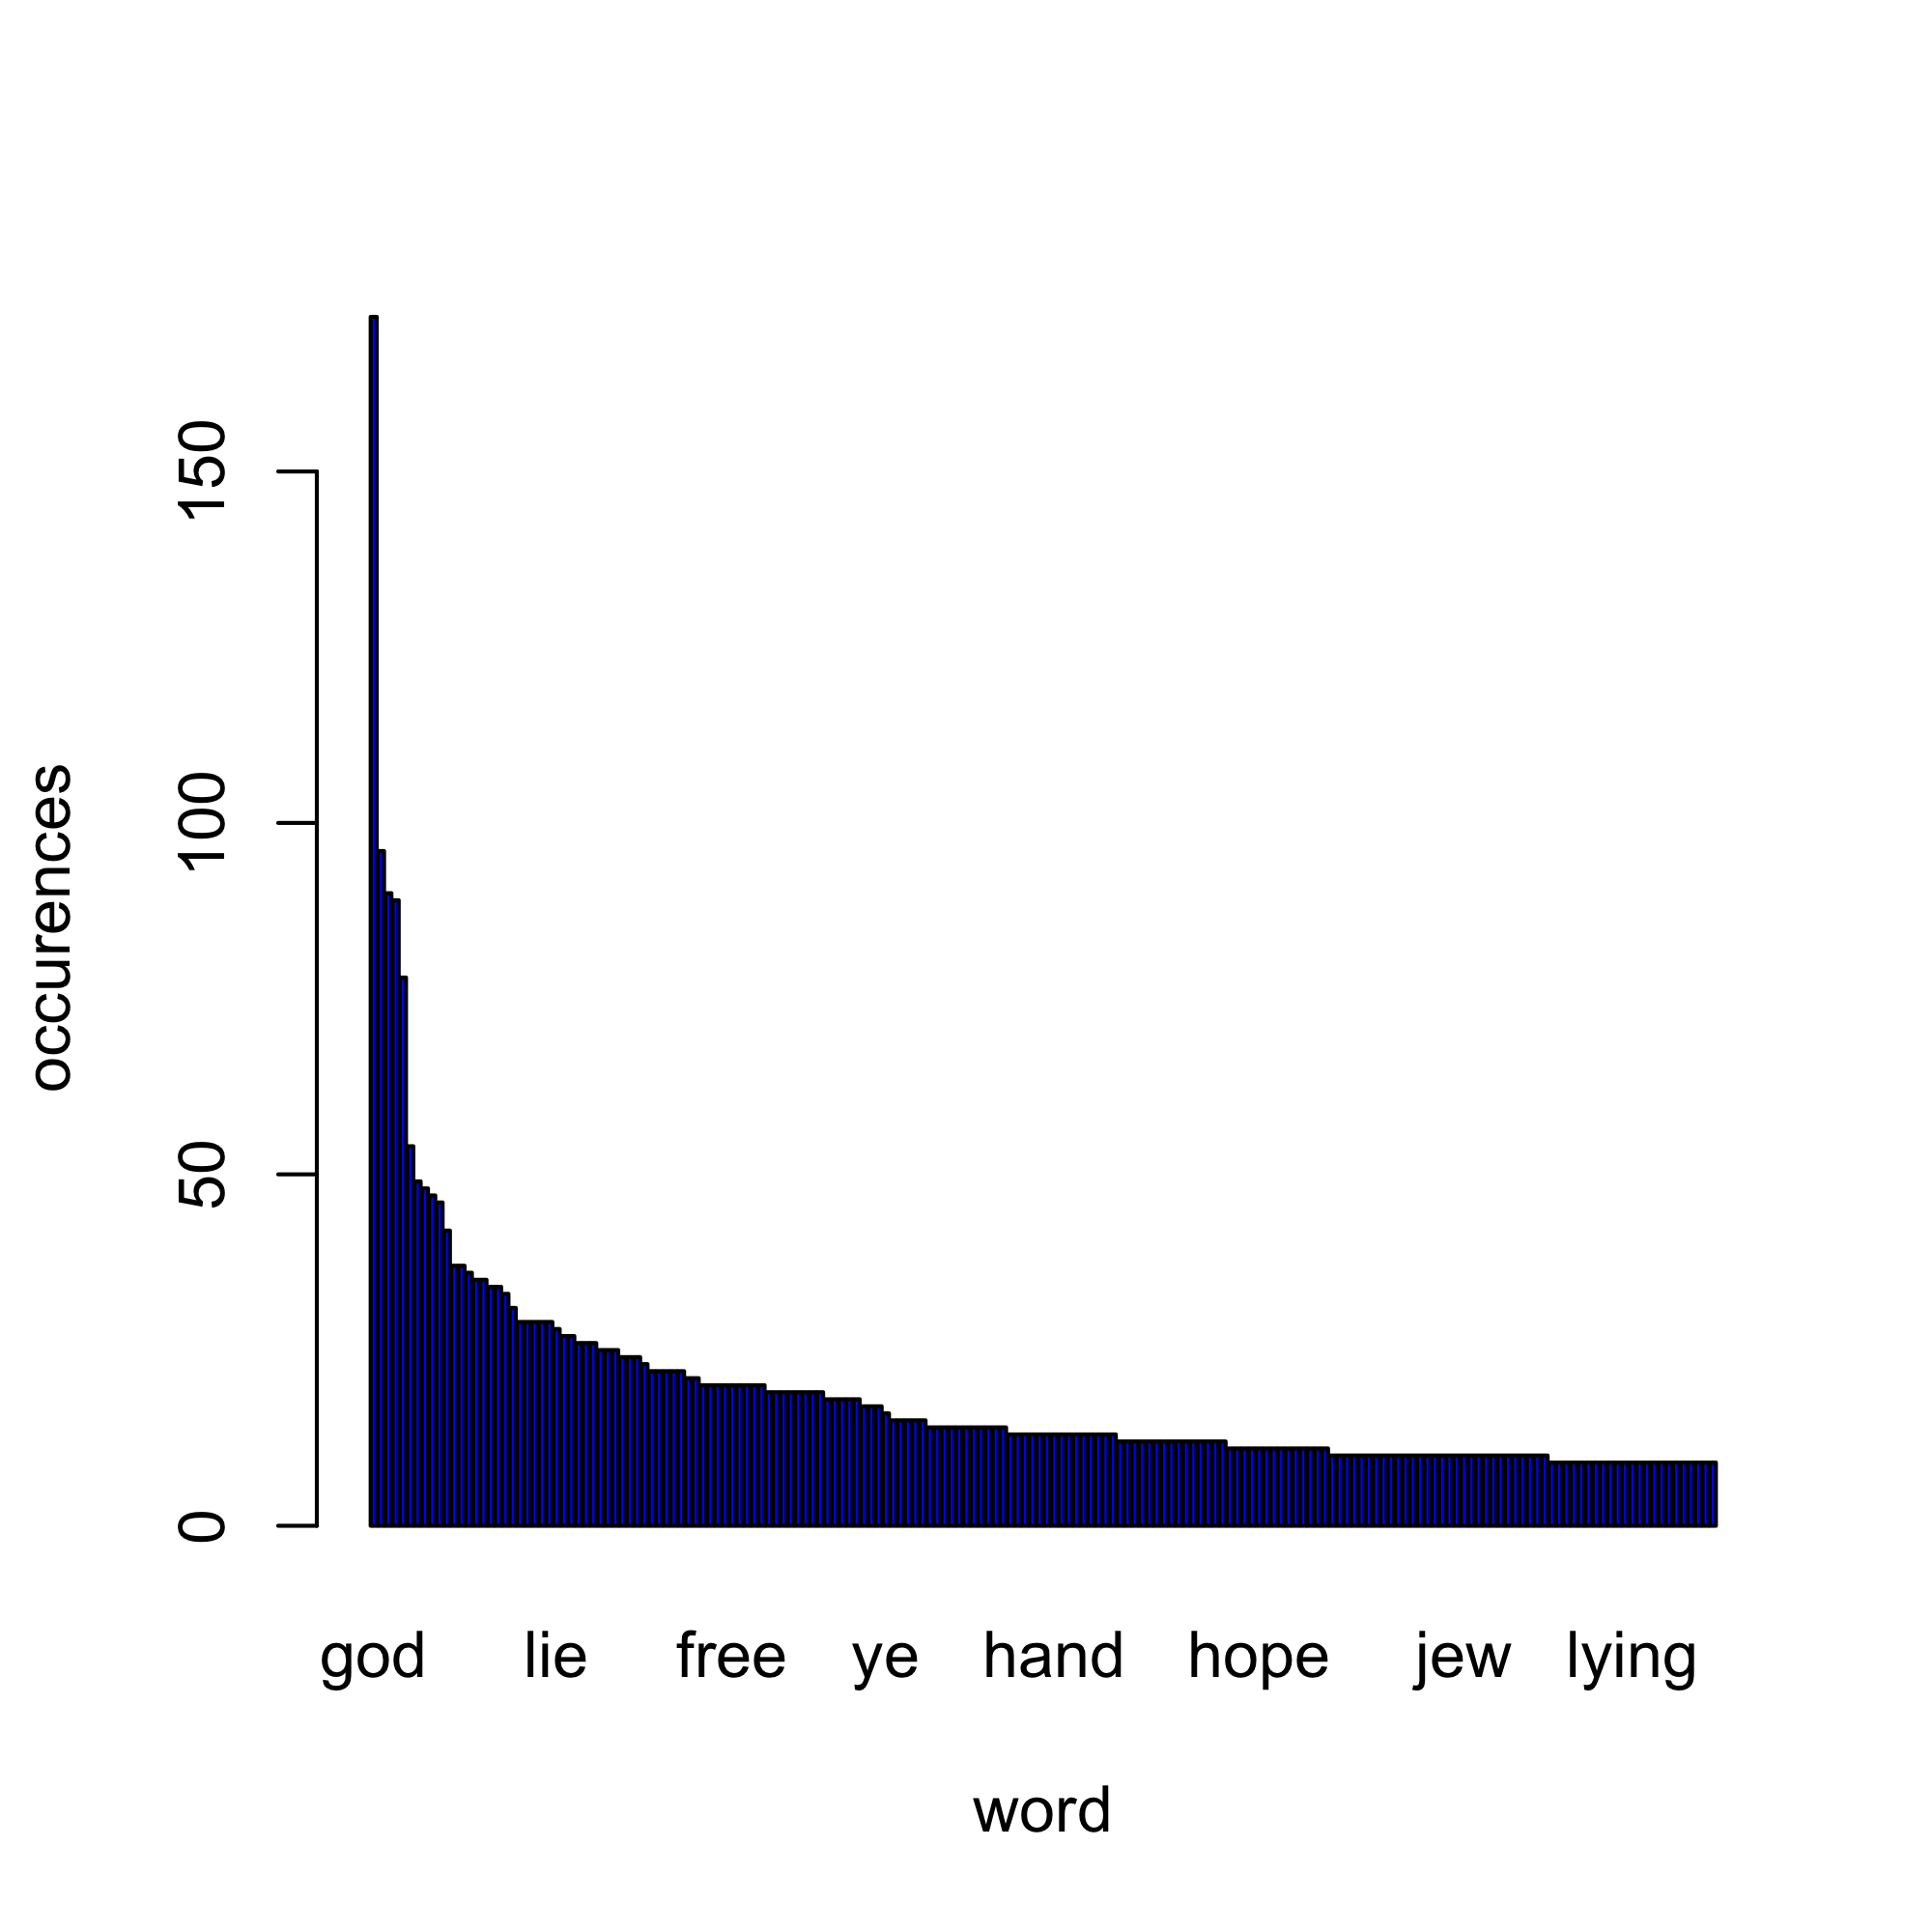
\includegraphics[width=\linewidth]{freq_words.png}
		\caption{Word occurrence in the book.}
		\label{fig:barplot_book}
	\end{subfigure}
	\begin{subfigure}[b]{0.45\linewidth}
		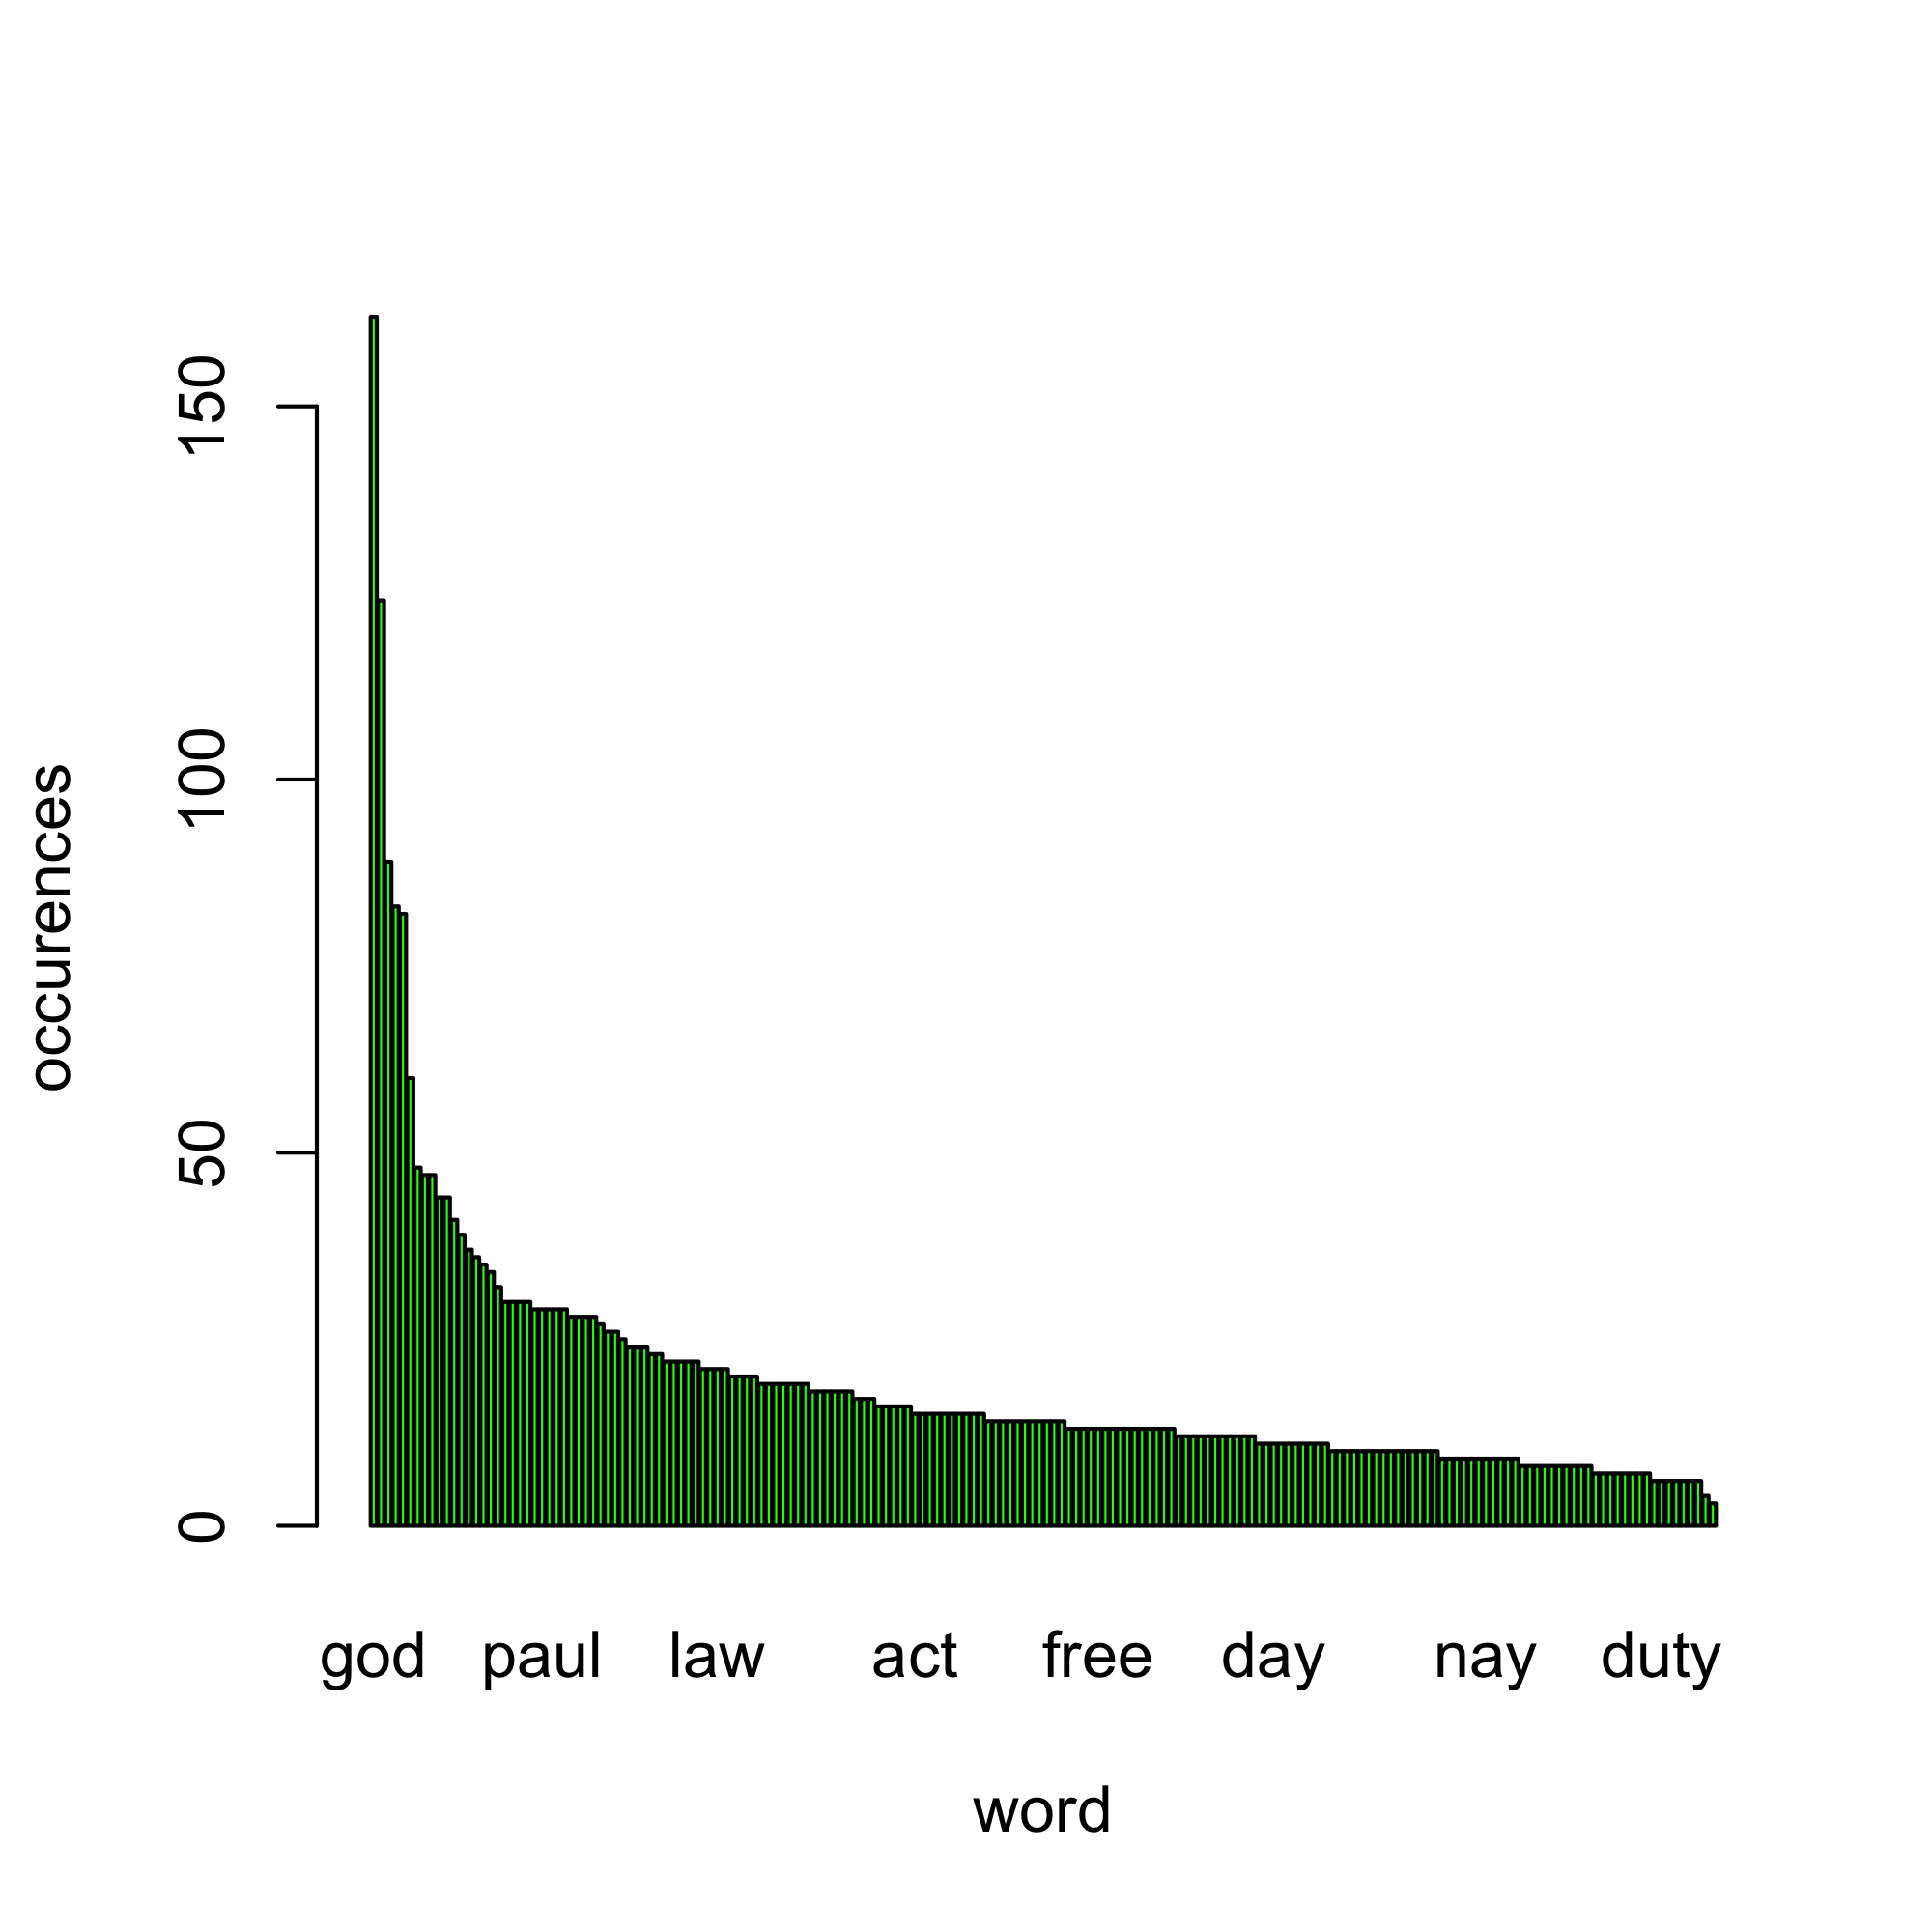
\includegraphics[width=\linewidth]{random_words.png}
		\caption{Word occurrence of words pseudo-randomly selected from the book.}
		\label{fig:barplot_random}
	\end{subfigure}
	\caption{Barplots of word occurrences.} 
	\label{fig:barplots}
\end{figure}

\begin{figure}
\centering
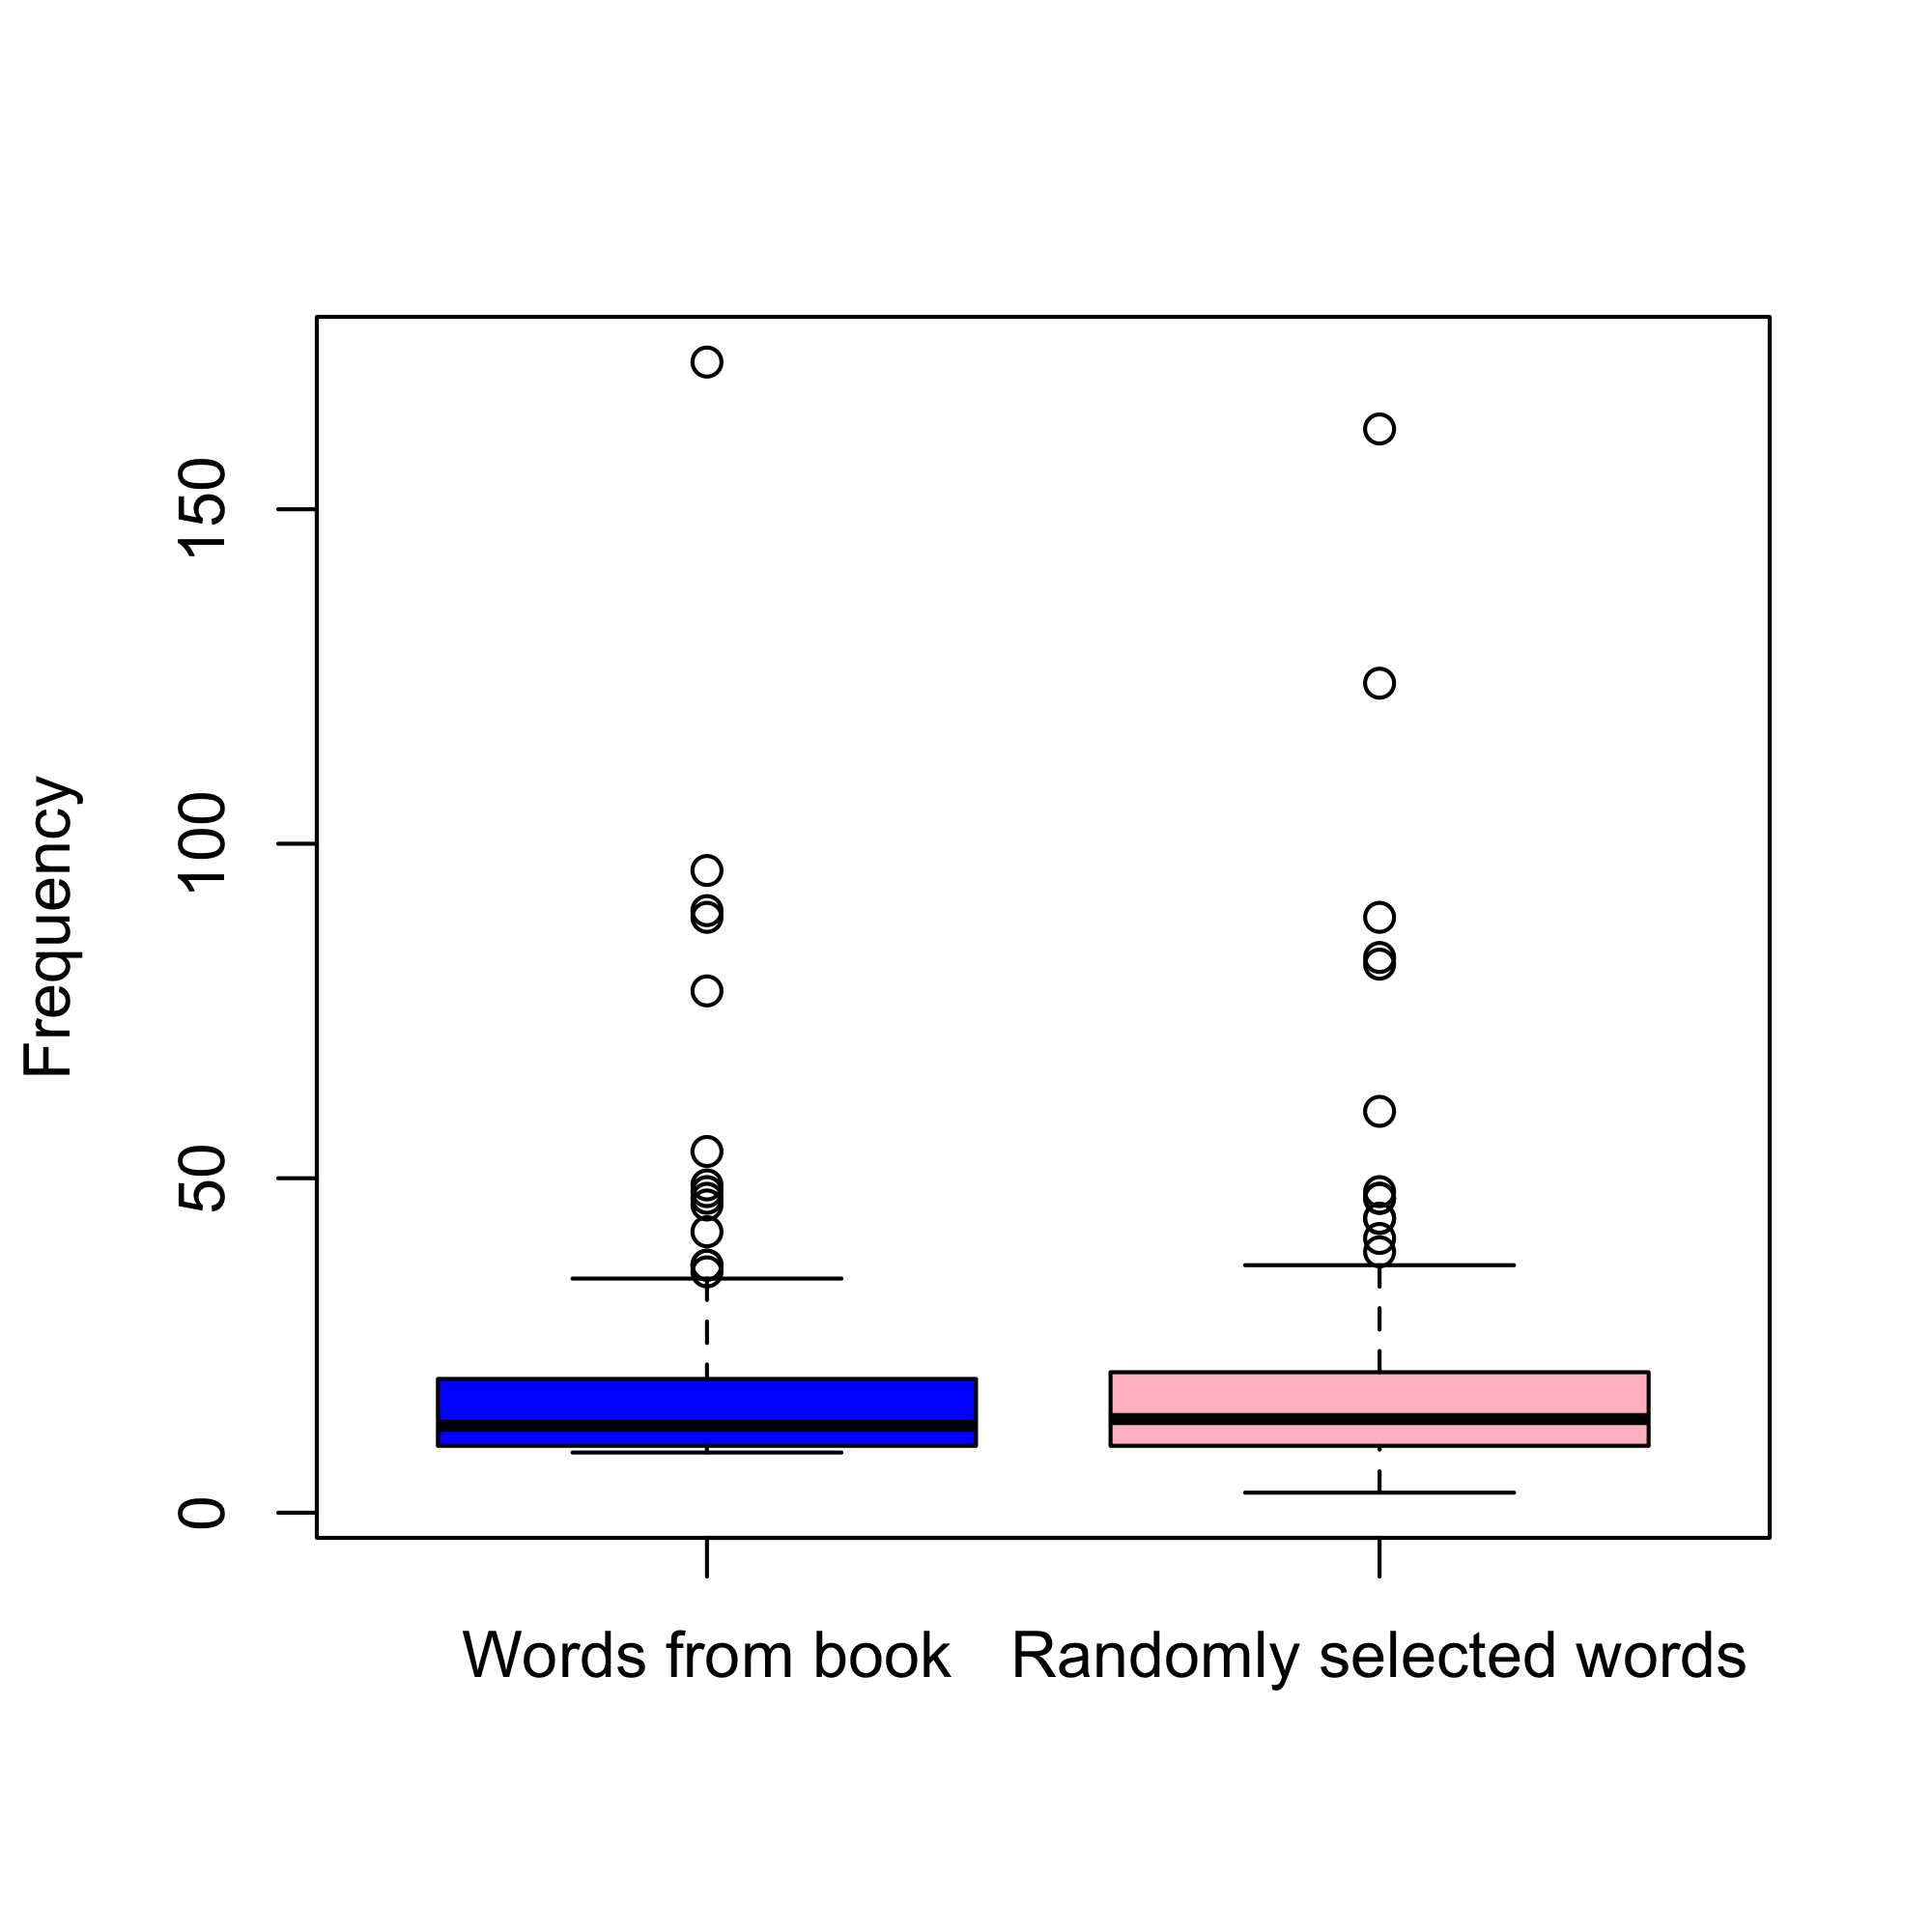
\includegraphics[width=.5\linewidth]{boxplot_words.png}
\caption{Comparison of word frequency.}
\label{fig:boxplot}
\end{figure}

\subsection{Network representation}
In a previous text analysis\footnote{It can be found at \url{https://github.com/palafox794/AppliedProbabilityModels/tree/master/Assignment2}}, a network representation of our book was made, as is seen in Figure \ref{fig:book-network}. Using R's library \texttt{igraph}, function \texttt{sample\_degseq}, we create a random network which has the same degrees as our book network. This is done based on the configuration model \cite{newman}, discarding graphs with multiple-edges or self-loops. We cannot say much about how these two compare, but decided to show them here nonetheless. The networks are shown side by side in Figure \ref{fig:network}.

\begin{figure}
	\centering
	\begin{subfigure}{0.45\linewidth}
		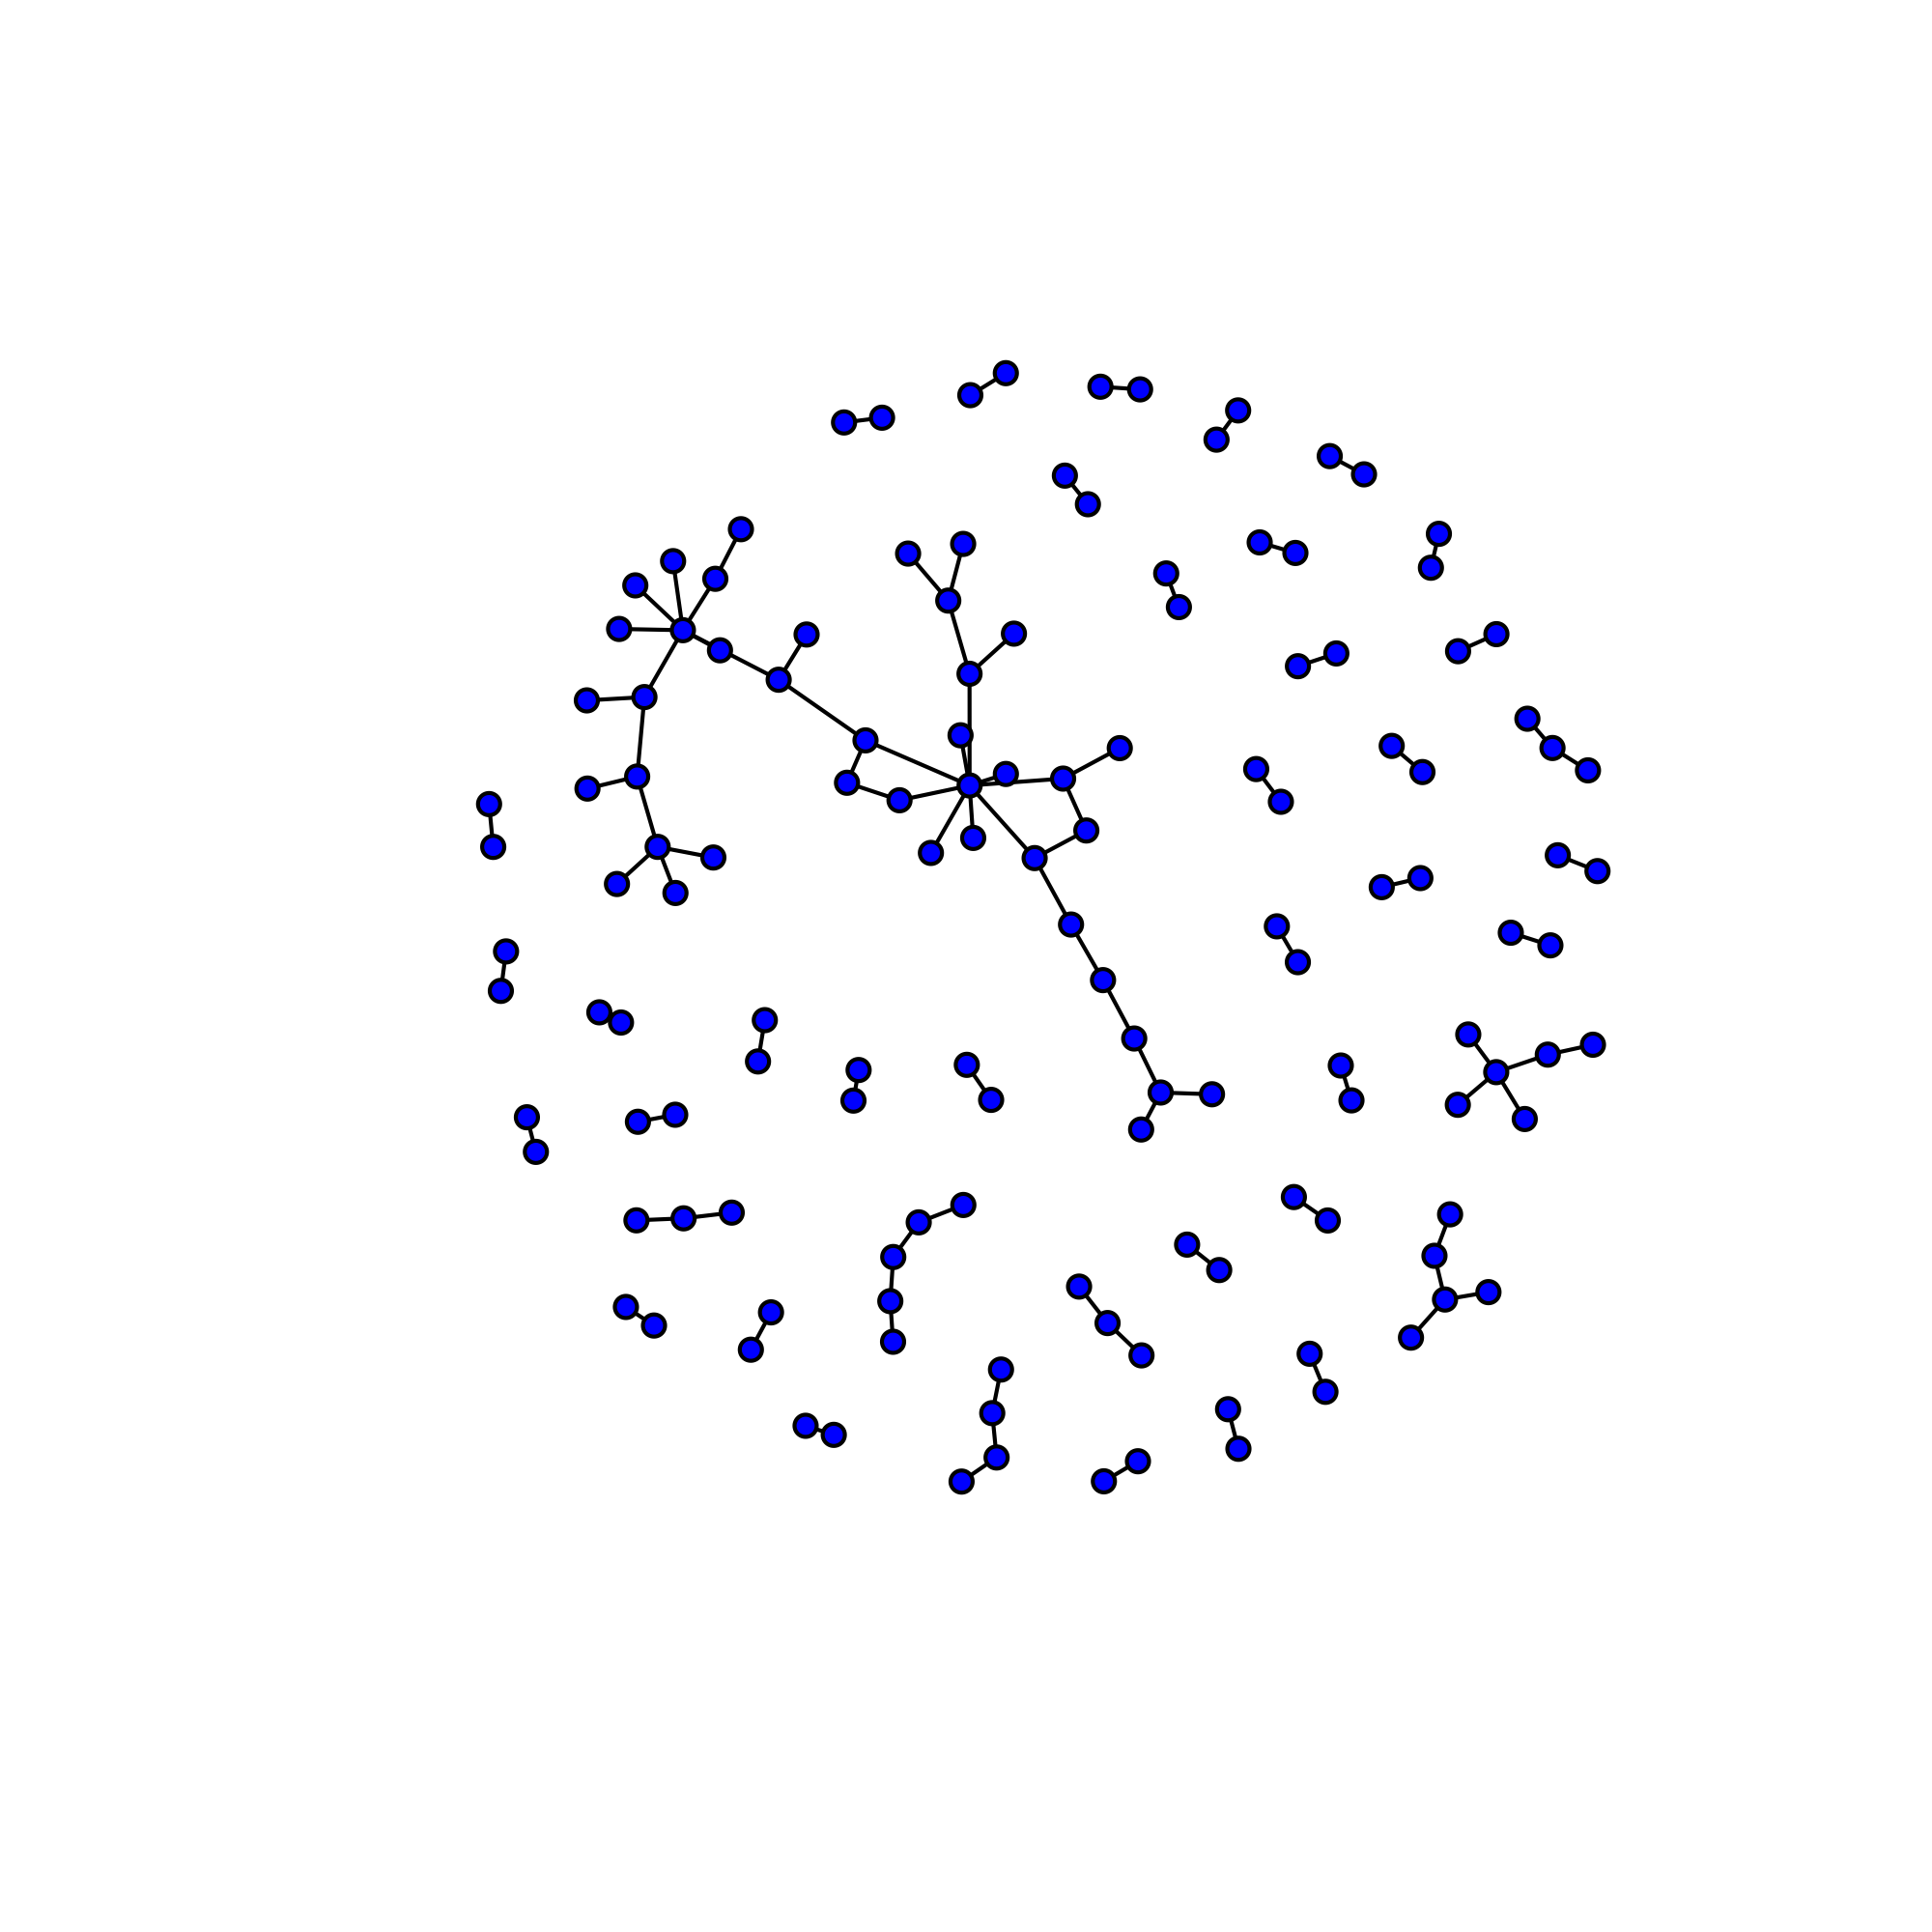
\includegraphics[width=\linewidth]{book_network.png}
		\caption{Book network. Words are vertices and edges joining words appear as a bigram in the text.}
		\label{fig:book-network}
	\end{subfigure}
	\hfill
	\begin{subfigure}{0.45\linewidth}
		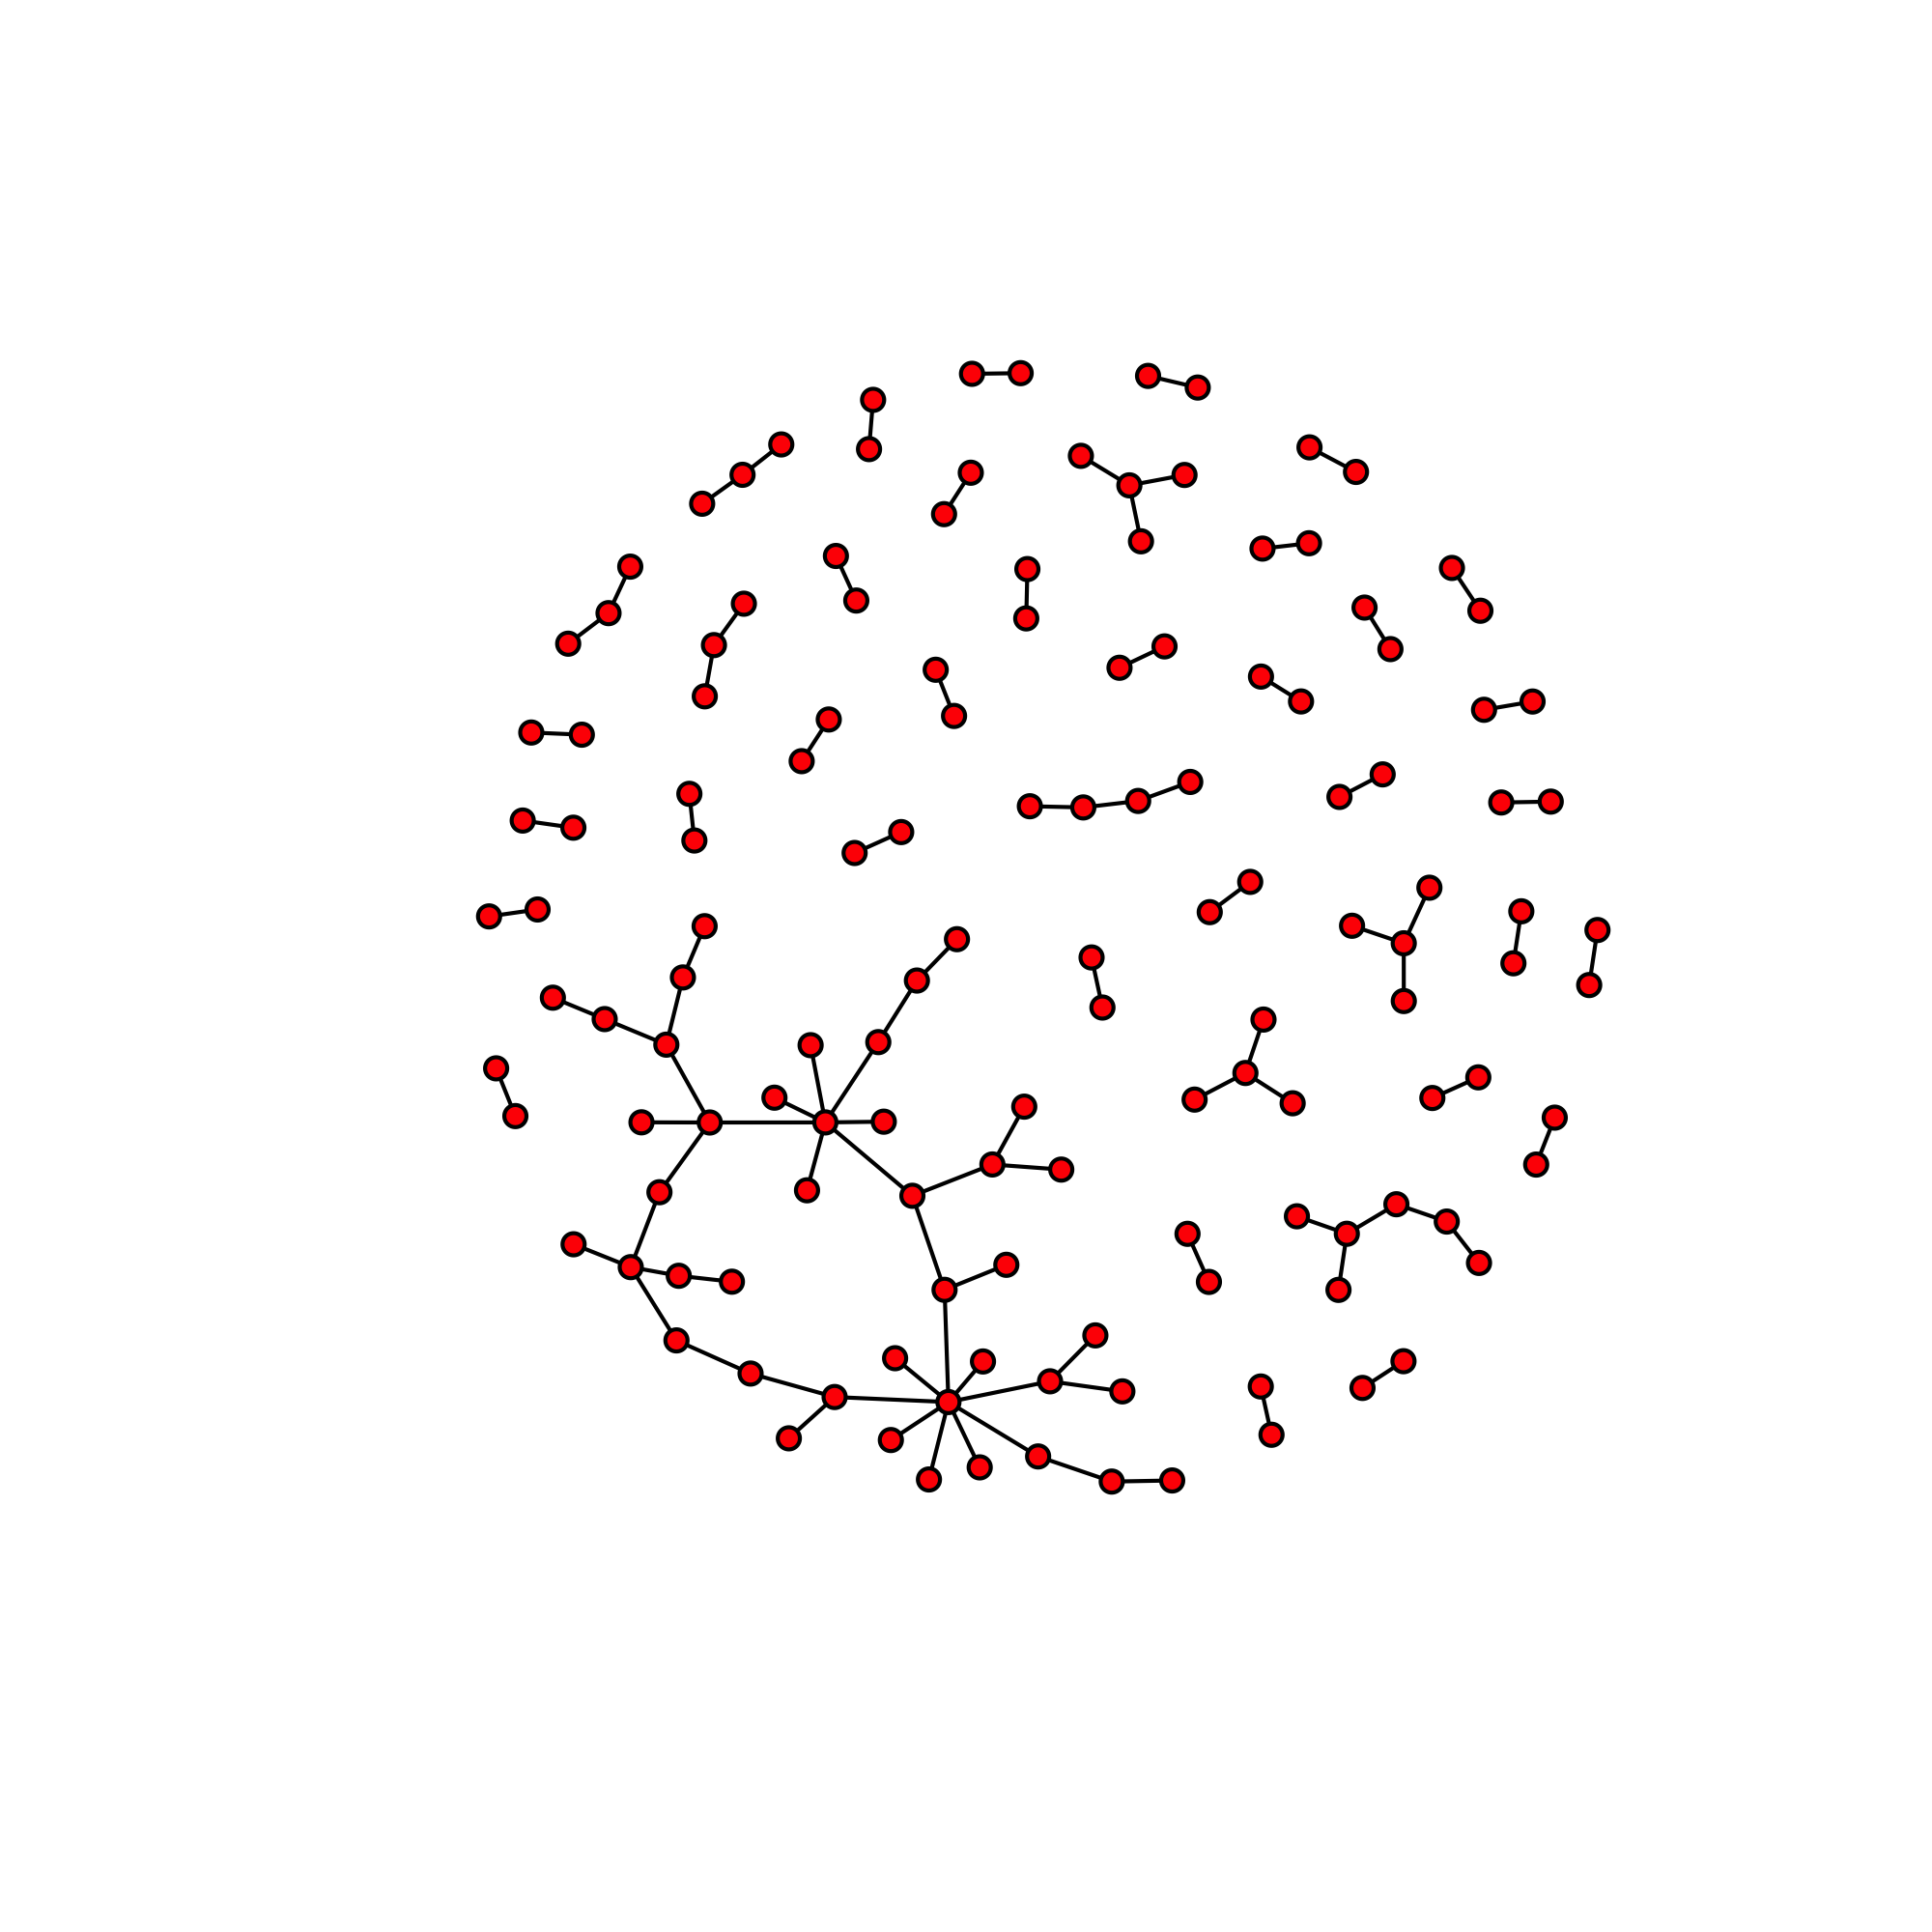
\includegraphics[width=\linewidth]{random_network.png}
		\label{fig:random-network}
		\caption{Random network with same degree distribution as book network.}
	\end{subfigure}
   	\caption{Network representation.} 
	\label{fig:network}
\end{figure}


\section{Conclusion}
Overall, our exposition is very elementary. Further statistical analysis can be done to determine whether the geometric distribution really is a good fit for the sentences' length distribution. A deeper study of discrete probability distributions may help find a good fit for the distribution of how frequent words distribute in the text. More sophisticated network analysis techniques could be deployed, aiming to understand the differences and similarities of our book network and a random network with the same degree sequence.

%%%%%%%%%%%%%%%%%%%%%%%%%%%%

\bibliographystyle{acm}
\bibliography{refr}


%%%%%%%%%%%%%%%%%%%%%%%%%%%%
\end{document}
